\red{à fusionner avec annexe C sur l'approximation géométrique}
\ETT fonctionne à partir d'un maillage, et non pas de la géométrie exacte du système modélisé. Ce qui est une source non négligeable d'erreur pour des géométries courbées. L'exemple développé dans cette sous partie est celui de deux cercles concentriques, de rayons de 100~$u.a.$ et 200~$u.a.$. Il a été choisi car il permet de voir directement l'erreur commise sur les facteurs de vue. En effet, d'une manière analgoue à celle développée plus tôt dans la Section \ref{part:calcul_anal}, le ratio les facteurs de vue sont directement liés au ratio des périmètres: $F_{outer \rightarrow inner}= \frac{P_{inner}}{P_{outer}}$. 


Le Tableau~\ref{tab:err_ratio_perimeter} présente les erreurs relatives obtenues pour les trois niveaux de discrétisation des cercles utilisés dans cette étude. La formule de l'erreur géométrique est développée dans l'Annexe \ref{anx:cc}.

\begin{table}[H]
\centering
\begin{tabular}{ccccc}
\toprule
$N_{inner}$ & $N_{outer}$ &
$P_ {inner}^{(N)}/P_{outer}^{(N)}$ &
Erreur géométrique (\%) &
Erreur \ETT (\%)\\
\midrule
12  & 14   & 0.488793 & $2.2\times10^{-2}$ & $2.8\times10^{-3}$ \\
79  & 157  & 0.499934 & $1.3\times10^{-4}$ & $2.0\times10^{-4}$ \\
628 & 1000 & 0.499997 & $6.3\times10^{-6}$ & $2.5\times10^{-6}$ \\
\bottomrule
\end{tabular}
\caption{Comparaison entre l'erreur géométrique sur le rapport des périmètres et l'erreur observée sur les facteurs de vue.}
\label{tab:err_ratio_perimeter}
\end{table}

\begin{figure}[H]
\centering

\begin{minipage}[t]{0.32\textwidth}
\centering
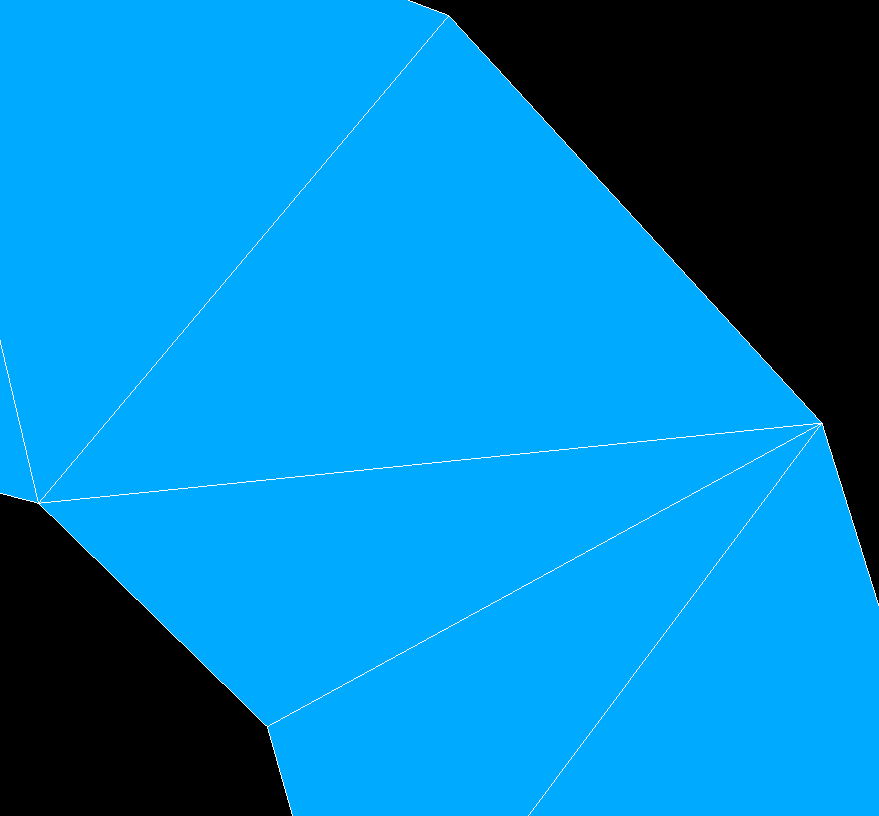
\includegraphics[width=0.66\linewidth]{PICTURES/c2/circles_Coarse.png}

\small\textbf{(a) Maillage très grossier}
\end{minipage}
\hfill
\begin{minipage}[t]{0.32\textwidth}
\centering

\includegraphics[width=0.66\linewidth]{PICTURES/c2/circles_coarse.png}

\small\textbf{(b) Maillage  raffiné}
\end{minipage}
\hfill
\begin{minipage}[t]{0.32\textwidth}
\centering
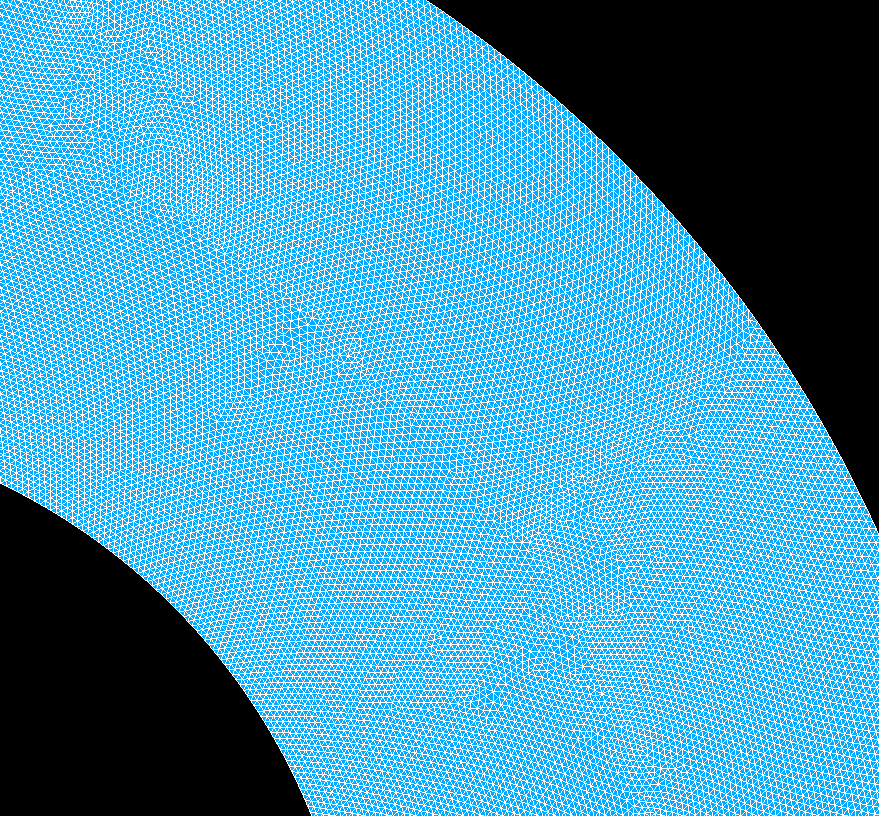
\includegraphics[width=0.66\linewidth]{PICTURES/c2/circles_fine.png}

\small\textbf{(c) Maillage très raffiné}
\end{minipage}


\end{figure}

Ces résultats montrent que l'erreur géométrique induite par la discrétisation du contour décroît rapidement avec le raffinement du maillage. Alors que le maillage le plus grossier conduit à une erreur de l'ordre de $2\,\%$ sur le rapport des périmètres, celle-ci devient inférieure à $10^{-4}$ dès le second niveau de discrétisation et devient satisfaisant pour le maillage le plus fin. Il faut garder en tête le problème d'hyper sensibilité évoqué au Paragraphe \ref{part:hypersens} et insister sur l'importance de la précision des facteurs de vue.


